\chapter{Einleitung}
\label{chap:einleitung}

\begin{figure}[!h] \centering
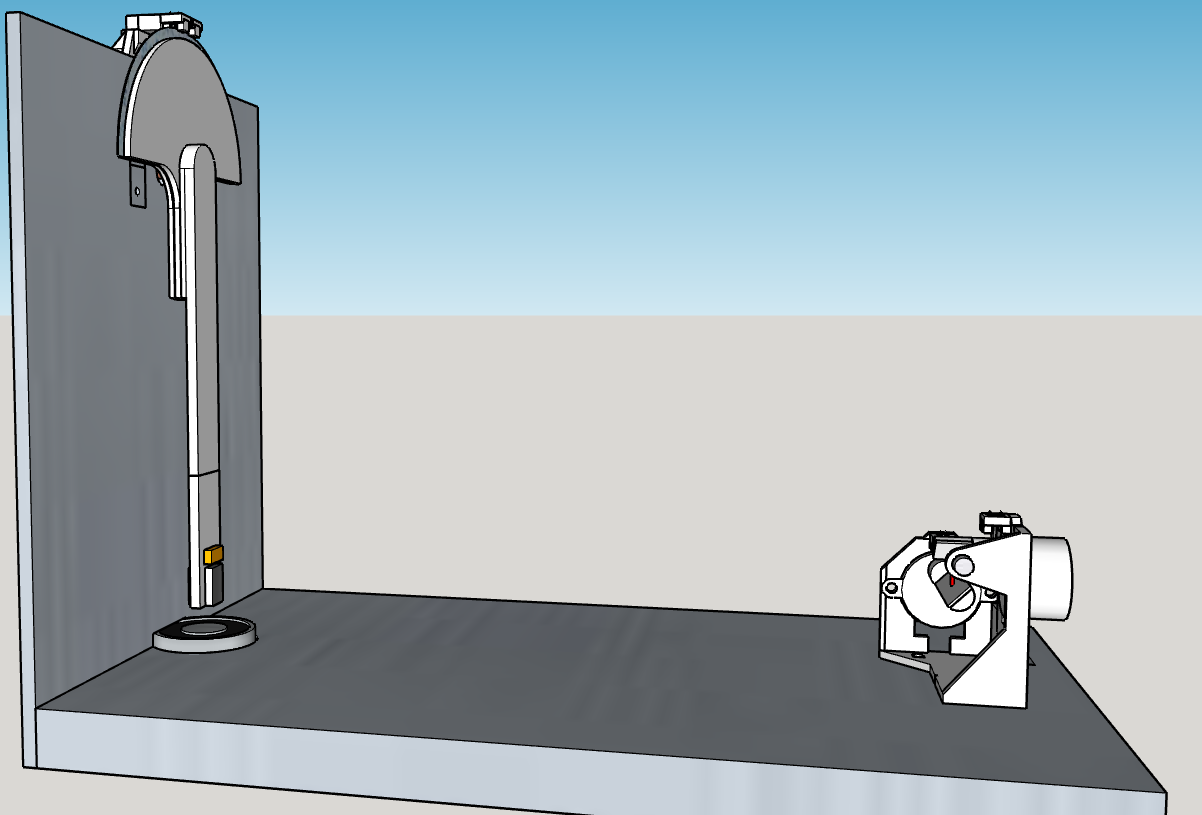
\includegraphics[width=0.7\textwidth]{img/Sketchup/Pendel03.PNG}
\caption{3D-Modell einer Spiegelablenkeinheit und einem Pendel.}
\label{fig:3dPendel}
\end{figure}


In der Lehrveranstaltung "`Mikrocomputer Labor"' sollen Studierende den Umgang mit Mikrocontrollern auf spielerische Art und Weise erlernen.
Diese Aufbauten beinhalten meistens verschiedene Sensoren, Aktuatoren, Eingabe- und Ausgabegeräte.
Da für diese Lehrveranstaltung immer wieder neue Aufbauten mit Mikrocontrollern benötigt werden, wurde ich von einem Betreuer des Labors beauftragt, einen neuen Prototypen zu entwerfen.
Die Vorgaben für diesen Prototyp sind, dass eine Laserablenkeinheit enthalten ist, welche auf ein Objekt gerichtet ist.
Wichtige Eigenschaften eines solchen Laboraufbaus sind, dass er optisch ansprechend ist und einer Fehlbedienung mechanisch und elektrisch über einen langen Zeitraum standhält.

Auch an die Aufgabenstellung, welche durch den Prototypen gestellt wird, richten sich verschiedene Anforderungen.
Dabei ist es wichtig, dass diese leicht erklärbar und gut vorstellbar ist.
Sie darf weder über- noch unterfordern und es müssen verschiedene Teile aus verschiedenen Disziplinen vorhanden sein, um die Aufgabe interessant zu machen.
So können Teilaufgaben sowohl aus den Gebieten der Mathematik, Informatik, Regelungstechnik als auch aus anderen entspringen.
Einige Eigenschaften sind mit der Vorgabe der Spiegelablenkeinheit schon erfüllt, auf die weiteren gilt es besonders Acht zu geben.

Als Ziel für den zu steuernden Laserpunkt kommen sowohl feststehende Objekte als auch bewegliche infrage.
Um die Dynamik zu erhöhen und somit die Aufgabe interessanter zu machen, ist die Auswahl auf ein schwingendes oder sich drehendes Objekt gefallen.
Die erste Realisierung wurde dabei mit einem Pendel bewerkstelligt.
Ein Beispiel für diesen Aufbau ist in Abbildung~\ref{fig:3dPendel} zu sehen.
Um die Zielgenauigkeit zu detektieren, besitzt das Pendel einen Detektor für den Laserstrahl.
Dies macht die Aufgabe sehr interessant, da mit dieser Information auch eine Regelung und nicht nur eine Steuerung realisierbar ist.

Eine Regelung eines Lasers auf ein Ziel ist eine sehr interessante Aufgabe, vor allem deswegen, da dies kein Standardalgorithmus ist, welcher in der Literatur vollständig vorhanden ist.
Um einen solchen Prototypen aufzubauen und die nötige Software zu erarbeiten, sind verschiedene Probleme zu lösen.
Die Methodik, wie in dieser Arbeit auf die verschiedenen Teile eingegangen wird, gliedert sich in jeweils einen Abschnitt über den Aufbau, die Elektronik und einen abschließenden für die Software.


% Einleitung
% - Weshalb ist das Problem interessant?
% - - Microcomputer labor
% - Was ist das Neue, was das Herausfordernde an der Arbeit?
% - - Neu: Laserablenkeinheit
% - Was ist Ihr eigener Beitrag (Contribution)?
% - - Auswahl der Verfahren
% - Wie sieht die Methodik aus?
% - - Hardware, Elektronik, Software
% - Welche Aufgabenstellung wird verfolgt?
% - - Prototyp mit Laser

% * Leser Hat Kurzfassung nicht gelesen
% * Versprechen abgeben, das mit der Arbeit erarbeitet, bewiesen wird
% * Roter Faden beginnt



% Kurzfassung:
% Was ist das Problem?
% Wie sieht der Lösungsansatz aus? Welche wesentliche Idee („Key Idea“) steckt dahinter?
% Was ist die Lösung? Was bewirkt die Lösung? Was folgt aus der Lösung?
% Was sind die wichtigsten Ergebnisse und Erkenntnisse?
